% =====================================================================
\section{Quiz 2: Complete Solutions}\label{ch:quizsol}
% =====================================================================

Each problem below is solved in full, in the way it should be written on the
exam: every step says \emph{what} we do, \emph{why} we do it, and shows the
complete computation. After the full solution you will find:
\begin{itemize}
\item an \textbf{Alternative method (optional)} box, a faster route you may use
      to \emph{check} your answer (the full method is what you should write);
\item \textbf{Traps}, the mistakes that cost points;
\item \textbf{If they change it}, how the same problem could appear differently.
\end{itemize}

% ---------------------------------------------------------------------
\subsection{Problem 1: a curve of intersection (22 points)}

\textbf{What the problem tests.} Parametrizing the curve where two surfaces meet,
with a prescribed starting point and orientation (Slides~5, Example~5.4), and
then using that parametrization for a tangent line, an arc length and a
curvature. All four parts depend on part~(a), so part~(a) must be checked
carefully before continuing.

\subsubsection*{(a) Finding $\vr(t)$ [6 points]}

\step{1}{Decide which variable to eliminate.}
The orientation is described ``when viewed from above the $xy$-plane'', that is,
by looking at how the shadow of the curve on the $xy$-plane moves. So we want
to describe the curve through its $x$- and $y$-coordinates, and we eliminate
$z$. The plane is the simpler surface, and it is easy to solve for $z$:
\[
  3x-4z=0\quad\Longrightarrow\quad 4z=3x\quad\Longrightarrow\quad z=\frac{3x}{4}.
\]

\step{2}{Substitute into the sphere to get the shadow of the curve.}
Every point of $C$ lies on the sphere, so its coordinates satisfy
$x^2+y^2+z^2=25$. Replacing $z$ by $\frac{3x}{4}$:
\[
  x^2+y^2+\left(\frac{3x}{4}\right)^2=25
  \;\Longrightarrow\; x^2+\frac{9x^2}{16}+y^2=25
  \;\Longrightarrow\; \frac{16x^2+9x^2}{16}+y^2=25
  \;\Longrightarrow\; \frac{25x^2}{16}+y^2=25 .
\]
Dividing both sides by $25$ puts this in standard form:
\[
  \frac{x^2}{16}+\frac{y^2}{25}=1 .
\]
This equation contains no $z$, so it describes the ``shadow'' of $C$ on the
$xy$-plane: an ellipse with $a^2=16$ (so $a=4$, along the $x$-axis) and
$b^2=25$ (so $b=5$, along the $y$-axis).

\step{3}{Parametrize the shadow using the hint.}
The hint says that $\frac{x^2}{a^2}+\frac{y^2}{b^2}=1$ is parametrized by
$x=a\cos t$, $y=b\sin t$. With $a=4$ and $b=5$:
\[
  x=4\cos t,\qquad y=5\sin t,\qquad 0\le t\le2\pi .
\]
Let us confirm that this satisfies the ellipse equation:
$\frac{16\cos^2t}{16}+\frac{25\sin^2t}{25}=\cos^2t+\sin^2t=1$.\checkok

\step{4}{Recover $z$ from the plane.}
From Step~1, $z=\frac{3x}{4}=\frac{3}{4}\cdot4\cos t=3\cos t$. Putting the three
coordinates together:
\[
  \boxed{\vr(t)=\ip{4\cos t,\;5\sin t,\;3\cos t},\qquad0\le t\le2\pi .}
\]

\step{5}{Check every requirement of the problem.}
\begin{itemize}
\item \emph{The curve lies on the sphere:}
      $(4\cos t)^2+(5\sin t)^2+(3\cos t)^2=16\cos^2t+25\sin^2t+9\cos^2t
      =25\cos^2t+25\sin^2t=25$.\checkok
\item \emph{The curve lies on the plane:} $3(4\cos t)-4(3\cos t)=12\cos t-12\cos t=0$.\checkok
\item \emph{It starts at $P$:} at $t=0$, $\vr(0)=\ip{4\cdot1,\;5\cdot0,\;3\cdot1}=\ip{4,0,3}$.\checkok
\item \emph{It is counterclockwise from above:} as $t$ goes from $0$ to
      $\frac\pi2$, $\pi$, $\frac{3\pi}{2}$, the shadow $(4\cos t,5\sin t)$ goes from
      $(4,0)$ to $(0,5)$, $(-4,0)$, $(0,-5)$. Moving from the positive $x$-axis to
      the positive $y$-axis is the counterclockwise sense.\checkok
\end{itemize}

\begin{altmethod}
Because the plane $3x-4z=0$ passes through the centre $(0,0,0)$ of the
sphere, the curve $C$ is a \emph{great circle}: a circle of radius $5$ (the
radius of the sphere) centred at the origin. In fact our answer can be written
\[
  \vr(t)=\cos t\,\ip{4,0,3}+\sin t\,\ip{0,5,0}
  =5\left[\cos t\,\ip{\tfrac45,0,\tfrac35}+\sin t\,\ip{0,1,0}\right],
\]
and the two vectors in brackets are perpendicular unit vectors, which is
exactly the form of a circle of radius $5$. Knowing this lets you predict the
answers to (b)--(d) and check them: constant speed $5$, arc length equal to
$5$ times the angle swept, and curvature $\frac15$.
\end{altmethod}

\trap{(1) Writing $x=4\cos t$, $y=-5\sin t$: this is \emph{clockwise} from above.
(2) Writing $x=4\sin t$, $y=5\cos t$: this starts at $(0,5,0)$, not at $P$.
(3) Forgetting to write $z$ in terms of $t$.
(4) Dropping the term $\frac{9x^2}{16}$ and getting the circle $x^2+y^2=25$.}

\variant{\emph{Clockwise} from above, starting at $P$: $\vr(t)=\ip{4\cos t,\,-5\sin t,\,3\cos t}$.
Starting at $(-4,0,-3)$, counterclockwise: $\vr(t)=\ip{-4\cos t,\,-5\sin t,\,-3\cos t}$.
A plane that does not pass through the centre (for example $z=x+1$) is handled in
exactly the same way, but the shadow is then an ellipse that is not centred at
the origin.}

\begin{figure}[H]
  \centering
  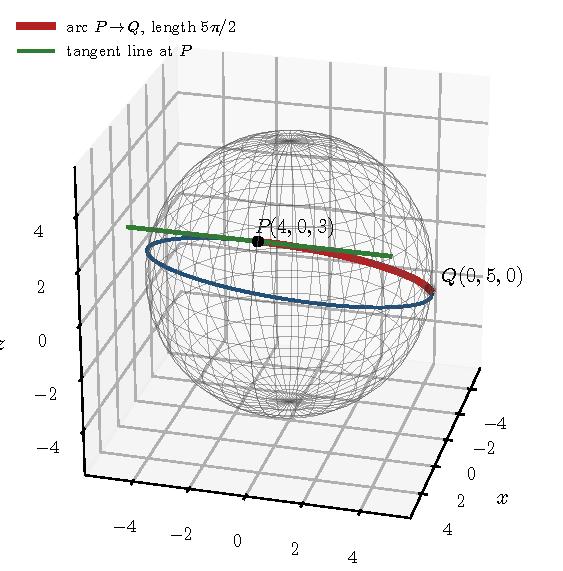
\includegraphics[width=0.56\linewidth]{great_circle}
  \caption{Problem 1: the curve $C$ (blue) is a great circle of the sphere of
  radius 5. Red: the counterclockwise arc from $P$ to $Q$ (one quarter of
  $C$). Green: the tangent line at $P$, parallel to $\vj$.}
  \label{fig:gc}
\end{figure}

\subsubsection*{(b) Tangent line at $P(4,0,3)$ [4 points]}

A line needs a point and a direction. The point is $P(4,0,3)$. The direction of
the tangent line is the tangent vector $\vr\,'(t)$ evaluated at the value of $t$
that gives $P$.

\step{1}{Differentiate $\vr(t)$ component by component.}
\[
  \vr\,'(t)=\ip{\frac{\dd}{\dd t}(4\cos t),\;\frac{\dd}{\dd t}(5\sin t),\;\frac{\dd}{\dd t}(3\cos t)}
  =\ip{-4\sin t,\;5\cos t,\;-3\sin t}.
\]
\step{2}{Find the parameter of $P$.} From part (a), $\vr(0)=\ip{4,0,3}$, so $P$ corresponds to $t=0$.
\step{3}{Evaluate the tangent vector there.}
$\vr\,'(0)=\ip{-4\sin0,\;5\cos0,\;-3\sin0}=\ip{0,\,5,\,0}$.
\step{4}{Write the line.} The vector equation of the line through $\vr_0=\ip{4,0,3}$
with direction $\vv=\ip{0,5,0}$ is $\mathbf L(s)=\vr_0+s\vv$:
\[
  \boxed{\mathbf L(s)=\ip{4,0,3}+s\ip{0,5,0}=\ip{4,\;5s,\;3},\qquad s\in\R .}
\]
Any nonzero multiple of the direction vector, such as $\ip{0,1,0}$, gives the same
line and is equally correct.

\begin{altmethod}
For a circle, the tangent at a point is perpendicular to the radius to that
point, $\ip{4,0,3}$, and it lies in the plane of the circle, whose normal is
$\ip{3,0,-4}$. A vector perpendicular to both is their cross product:
\[
  \ip{4,0,3}\times\ip{3,0,-4}=\ip{0\cdot(-4)-3\cdot0,\;3\cdot3-4\cdot(-4),\;4\cdot0-0\cdot3}=\ip{0,25,0},
\]
which is parallel to $\ip{0,5,0}$, in agreement with the derivative.
\end{altmethod}

\trap{Giving only the direction vector (not a line), or writing the line through
the origin, $s\ip{0,5,0}$, instead of through $P$.}

\subsubsection*{(c) Arc length from $P$ to $Q(0,5,0)$ [5 points]}

The arc length from $t=t_1$ to $t=t_2$ is $L=\displaystyle\int_{t_1}^{t_2}\norm{\vr\,'(t)}\,\dd t$.
We need the speed $\norm{\vr\,'(t)}$ and the parameter values of the two endpoints.

\step{1}{Compute the speed.} Using $\vr\,'(t)=\ip{-4\sin t,\,5\cos t,\,-3\sin t}$ from (b):
\[
  \norm{\vr\,'(t)}=\sqrt{(-4\sin t)^2+(5\cos t)^2+(-3\sin t)^2}
  =\sqrt{16\sin^2t+25\cos^2t+9\sin^2t}.
\]
Combine the two $\sin^2t$ terms: $16\sin^2t+9\sin^2t=25\sin^2t$. Therefore
\[
  \norm{\vr\,'(t)}=\sqrt{25\sin^2t+25\cos^2t}=\sqrt{25(\sin^2t+\cos^2t)}=\sqrt{25}=5 .
\]
The speed is constant.

\step{2}{Find the parameter of $Q(0,5,0)$.} We need $4\cos t=0$, $5\sin t=5$ and
$3\cos t=0$. The second equation gives $\sin t=1$, so $t=\frac\pi2$; then
$\cos\frac\pi2=0$, so the first and third equations hold as well.
\step{3}{Respect the orientation.} The curve is traversed counterclockwise,
which is the direction of increasing $t$. Starting at $P$ ($t=0$) and moving
forward we reach $Q$ at $t=\frac\pi2$. So $t$ runs from $0$ to $\frac\pi2$.
\step{4}{Integrate.}
\[
  L=\int_0^{\pi/2}5\,\dd t=5\Big[t\Big]_0^{\pi/2}=5\cdot\frac\pi2=\boxed{\frac{5\pi}{2}}\approx7.85 .
\]

\begin{altmethod}
Since $C$ is a circle of radius $5$ (see part (a)) and the arc from $P$ to $Q$
sweeps the angle $\frac\pi2$, i.e. one quarter of the circle, its length is
$\frac14\cdot2\pi\cdot5=\frac{5\pi}{2}$.
\end{altmethod}

\trap{(1) Going the wrong way round: integrating from $t=0$ backwards to
$t=-\frac{3\pi}{2}$ gives the \emph{clockwise} arc, of length $\frac{15\pi}{2}$.
(2) Not combining $16\sin^2t+9\sin^2t$; then the square root looks impossible to integrate.}

\subsubsection*{(d) Curvature at $P$ [7 points]}

We use the curvature formula for vector functions,
\[
  \kappa(t)=\frac{\norm{\vr\,'(t)\times\vr\,''(t)}}{\norm{\vr\,'(t)}^3},
\]
evaluated at $t=0$ (the parameter of $P$).

\step{1}{First derivative at $t=0$.} From (b), $\vr\,'(0)=\ip{0,5,0}$.
\step{2}{Second derivative.} Differentiating $\vr\,'(t)=\ip{-4\sin t,\,5\cos t,\,-3\sin t}$ once more:
\[
  \vr\,''(t)=\ip{-4\cos t,\;-5\sin t,\;-3\cos t},\qquad\vr\,''(0)=\ip{-4,\;0,\;-3}.
\]
\step{3}{Cross product.}
\[
  \vr\,'(0)\times\vr\,''(0)=\begin{vmatrix}\vi&\vj&\vk\\0&5&0\\-4&0&-3\end{vmatrix}
  =\vi\,\big(5\cdot(-3)-0\cdot0\big)-\vj\,\big(0\cdot(-3)-0\cdot(-4)\big)+\vk\,\big(0\cdot0-5\cdot(-4)\big)
  =\ip{-15,\;0,\;20}.
\]
\step{4}{Lengths.} $\norm{\ip{-15,0,20}}=\sqrt{225+0+400}=\sqrt{625}=25$, and
$\norm{\vr\,'(0)}^3=5^3=125$.
\step{5}{Curvature.}
\[
  \kappa(P)=\frac{25}{125}=\boxed{\frac15}.
\]

\begin{altmethod}
A circle of radius $R$ has curvature $\frac1R$ at every point, and $C$ is a circle
of radius $5$, so $\kappa=\frac15$ everywhere on $C$.
\end{altmethod}

\trap{Computing the curvature of the \emph{shadow} ellipse
$\frac{x^2}{16}+\frac{y^2}{25}=1$ at $(4,0)$ instead of the curvature of $C$. That
value is $\frac{4}{25}$, which is wrong: projecting a curve onto a plane changes
its curvature. Always differentiate the three-dimensional $\vr(t)$.}

% ---------------------------------------------------------------------
\subsection{Problem 2: directional derivative and maximum rate (13 points)}

\textbf{What the problem tests.} Computing partial derivatives of a function
built from three different kinds of terms, then the directional derivative
toward a point (Slides~6, Example~6.4) and the meaning of the gradient (the trio
activity).

\subsubsection*{Preliminary: the gradient at $P(1,1)$}

We need $f_x$ and $f_y$. We differentiate the function
$f(x,y)=2x^2y+\ln(x^2+y^2)+\dfrac{4x}{y}$ one term at a time.

\textbf{Partial derivative with respect to $x$} (treat $y$ as a constant):
\begin{itemize}
\item $\pd{}{x}\left(2x^2y\right)=2y\cdot2x=4xy$.
\item $\pd{}{x}\ln(x^2+y^2)=\dfrac{1}{x^2+y^2}\cdot\pd{}{x}(x^2+y^2)=\dfrac{2x}{x^2+y^2}$ (chain rule).
\item $\pd{}{x}\left(\dfrac{4x}{y}\right)=\dfrac{4}{y}$, because $\frac{4}{y}$ is a constant multiplying $x$.
\end{itemize}
So $f_x=4xy+\dfrac{2x}{x^2+y^2}+\dfrac4y$.

\textbf{Partial derivative with respect to $y$} (treat $x$ as a constant):
\begin{itemize}
\item $\pd{}{y}\left(2x^2y\right)=2x^2$.
\item $\pd{}{y}\ln(x^2+y^2)=\dfrac{2y}{x^2+y^2}$ (chain rule).
\item Write $\dfrac{4x}{y}=4x\,y^{-1}$. Then $\pd{}{y}\left(4x\,y^{-1}\right)=4x\cdot(-1)y^{-2}=-\dfrac{4x}{y^2}$.
\end{itemize}
So $f_y=2x^2+\dfrac{2y}{x^2+y^2}-\dfrac{4x}{y^2}$.

\textbf{Differentiability.} These partial derivatives are continuous wherever
$y\neq0$ (and $(x,y)\neq(0,0)$), in particular near $P(1,1)$. Hence $f$ is
differentiable at $P$, and we may use $\Du f=\grad f\cdot\vu$.

\textbf{Evaluate at $P(1,1)$.} Here $x^2+y^2=2$:
\[
  f_x(1,1)=4(1)(1)+\frac{2(1)}{2}+\frac41=4+1+4=9,\qquad
  f_y(1,1)=2(1)^2+\frac{2(1)}{2}-\frac{4(1)}{1^2}=2+1-4=-1 .
\]
Therefore $\grad f(1,1)=\ip{9,-1}$.

\subsubsection*{(a) Directional derivative from $P$ toward $Q$ [7 points]}

\step{1}{Direction vector.} ``From $P$ toward $Q$'' means the vector from $P$ to $Q$:
$\vecPQ=\ip{4-1,\;5-1}=\ip{3,4}$.
\step{2}{Make it a unit vector.} $\norm{\vecPQ}=\sqrt{3^2+4^2}=\sqrt{25}=5$, so
$\vu=\dfrac{\vecPQ}{\norm{\vecPQ}}=\ip{\dfrac35,\dfrac45}$.
\step{3}{Dot product with the gradient at $P$.}
\[
  \Du f(1,1)=\grad f(1,1)\cdot\vu=9\cdot\frac35+(-1)\cdot\frac45=\frac{27}{5}-\frac45=\boxed{\frac{23}{5}}.
\]
Interpretation: moving from $P$ toward $Q$, $f$ increases at the rate of
$\frac{23}{5}=4.6$ units per unit of distance.

\subsubsection*{(b) Unit vector of fastest increase [4 points]}

By the theorem on the maximum rate of change, $f$ increases most rapidly in the
direction of the gradient. To express this direction as a unit vector we divide
the gradient by its length. Since $\norm{\grad f(1,1)}=\sqrt{9^2+(-1)^2}=\sqrt{82}$,
\[
  \vu=\frac{\grad f(1,1)}{\norm{\grad f(1,1)}}=\boxed{\ip{\frac{9}{\sqrt{82}},\;-\frac{1}{\sqrt{82}}}}.
\]

\subsubsection*{(c) Maximum rate of increase [2 points]}

The maximum rate of increase is the length of the gradient:
$\norm{\grad f(1,1)}=\boxed{\sqrt{82}}\approx9.06$.

\textbf{Consistency check.} Every directional derivative must satisfy
$\abs{\Du f}\le\norm{\grad f}$. Here $\frac{23}{5}=4.6\le9.06$.\checkok

\trap{(1) Forgetting the chain-rule factor: $\pd{}{x}\ln(x^2+y^2)$ is
$\frac{2x}{x^2+y^2}$, not $\frac{1}{x^2+y^2}$.
(2) The sign of $\pd{}{y}\frac{4x}{y}$, which is negative.
(3) Not normalizing $\ip{3,4}$, which gives $23$ instead of $\frac{23}{5}$.
(4) Using $\ip{-3,-4}$ (the vector from $Q$ to $P$).
(5) In (b), answering $\ip{9,-1}$: the question asks for a \emph{unit} vector.
(6) In (c), answering with a vector: a rate is a number.}

\variant{\emph{Fastest decrease:} direction $-\frac{1}{\sqrt{82}}\ip{9,-1}=\ip{-\frac{9}{\sqrt{82}},\frac{1}{\sqrt{82}}}$,
rate $-\sqrt{82}$. \emph{Directions of zero change:} the unit vectors perpendicular
to $\ip{9,-1}$, namely $\pm\frac{1}{\sqrt{82}}\ip{1,9}$. \emph{Direction given by an angle
$\theta$:} $\Du f(1,1)=9\cos\theta-\sin\theta$.}

% ---------------------------------------------------------------------
\subsection{Problem 3: moving a given distance along a curve (5 points)}

\textbf{What the problem tests.} The arc-length function
$s(t)=\displaystyle\int_{t_0}^{t}\norm{\vr\,'(u)}\,\dd u$, which measures the distance travelled
along the curve from $t_0$ to $t$ (Slides~5, reparametrization by arc length).

\step{1}{Find the starting parameter.} We start at $(0,0,3)$. At $t=0$,
$\vr(0)=\ip{3\sin0,\;4\cdot0,\;3\cos0}=\ip{0,0,3}$, so the starting parameter is $t_0=0$.
\step{2}{Compute the speed.} $\vr\,'(t)=\ip{3\cos t,\;4,\;-3\sin t}$, so
\[
  \norm{\vr\,'(t)}=\sqrt{9\cos^2t+16+9\sin^2t}=\sqrt{9(\cos^2t+\sin^2t)+16}=\sqrt{9+16}=\sqrt{25}=5 .
\]
\step{3}{Write the distance travelled as a function of $t$.}
\[
  s(t)=\int_0^t\norm{\vr\,'(u)}\,\dd u=\int_0^t5\,\dd u=5t .
\]
\step{4}{Find when the distance equals $5$.} $s(t)=5\iff5t=5\iff t=1$. Since we
move in the direction of increasing $t$, we take this positive value.
\step{5}{Evaluate the position at $t=1$.}
\[
  \vr(1)=\ip{3\sin1,\;4(1),\;3\cos1}.
\]
\finalans{The new position is $\boxed{\left(3\sin1,\;4,\;3\cos1\right)}\approx(2.524,\;4,\;1.621)$,
where the angle $1$ is measured in \emph{radians}.}

\begin{altmethod}
When the speed is a constant $v$, distance $=v\times$(change in $t$). Here
$v=5$, so a distance of $5$ needs a change of $t$ of $\frac55=1$. The curve is a
helix of radius $3$ winding around the $y$-axis.
\end{altmethod}

\trap{(1) Evaluating $\vr(5)$: the parameter is not the distance (that point is
$25$ units away). (2) Computing $\sin1$ in degrees. (3) Stopping at ``$t=1$'':
the question asks for a position.}

\variant{Moving $5$ units in the direction of \emph{decreasing} $t$ gives $t=-1$ and the
point $(-3\sin1,\,-4,\,3\cos1)$. If the speed is not constant, for example for
$\vr(t)=\ip{e^t\cos t,e^t\sin t,e^t}$, then $s(t)$ is not a multiple of $t$ and one
must solve the equation $s(t)=$ distance (Predicted Problem~\ref{pp:arc}).}

% ---------------------------------------------------------------------
\subsection{Problem 4: curvature with an unknown constant (5 points)}

\textbf{What the problem tests.} The curvature formula
$\kappa=\dfrac{\norm{\vr\,'\times\vr\,''}}{\norm{\vr\,'}^3}$ applied to a plane curve, followed
by solving an equation that contains an absolute value.

\step{1}{Parametrize the parabola as a vector function.} The note asks for a
vector-valued parametrization. Using $x$ itself as the parameter, $x=t$ and
$y=at^2$. Because the cross product is defined only for vectors in space, we add
a zero $z$-component:
\[
  \vr(t)=\ip{t,\;at^2,\;0}.
\]
The origin corresponds to $t=0$.
\step{2}{First and second derivatives.}
\[
  \vr\,'(t)=\ip{1,\;2at,\;0},\qquad\vr\,''(t)=\ip{0,\;2a,\;0}.
\]
\step{3}{Cross product.}
\[
  \vr\,'\times\vr\,''=\begin{vmatrix}\vi&\vj&\vk\\1&2at&0\\0&2a&0\end{vmatrix}
  =\vi\,(2at\cdot0-0\cdot2a)-\vj\,(1\cdot0-0\cdot0)+\vk\,(1\cdot2a-2at\cdot0)=\ip{0,\;0,\;2a},
\]
whose length is $\sqrt{(2a)^2}=\abs{2a}=2\abs a$. (The square root of a square is an
absolute value.)
\step{4}{Speed at the origin.} $\norm{\vr\,'(0)}=\norm{\ip{1,0,0}}=1$, so $\norm{\vr\,'(0)}^3=1$.
\step{5}{Curvature at the origin.} $\kappa(0)=\dfrac{2\abs a}{1}=2\abs a$.
\step{6}{Solve the condition.} $2\abs a=4\iff\abs a=2\iff a=2$ or $a=-2$.

\finalans{$\boxed{a=2\ \text{or}\ a=-2}$.}

\why{$y=2x^2$ opens upward and $y=-2x^2$ opens downward, but they bend equally
sharply at the vertex. Curvature measures \emph{how much} a curve bends, not
in which direction, so both values work. The circle that best fits the
parabola at the vertex has radius $\frac1\kappa=\frac14$.}

\begin{altmethod}
For a graph $y=g(x)$ there is the formula $\kappa=\dfrac{\abs{g''(x)}}{\left(1+g'(x)^2\right)^{3/2}}$.
With $g=ax^2$: $g'(0)=0$ and $g''(0)=2a$, so $\kappa(0)=\abs{2a}$. This is a check only;
the problem explicitly asks for the vector method.
\end{altmethod}

\trap{Answering only $a=2$ (the question asks for \emph{all} values), or dropping
the absolute value and writing $2a=4$.}

% ---------------------------------------------------------------------
\subsection{Problem 5: directions with a prescribed directional derivative (5 points)}

\textbf{What the problem tests.} Solving $\grad f\cdot\vu=c$ for an unknown
\emph{unit} vector $\vu$ (Lecture Notes No.~6, Example~3.8).

\step{1}{Gradient at $(1,1)$.} $f_x=2x+y$ and $f_y=2y+x$, so
$\grad f(1,1)=\ip{2+1,\;2+1}=\ip{3,3}$.
\step{2}{Set up the unknowns.} Let the unknown unit vector be $\vu=\ip{a,b}$. Two
conditions must hold:
\begin{itemize}
\item the directional derivative is $3$: $\;\grad f(1,1)\cdot\vu=3a+3b=3$, i.e. $a+b=1$;
\item $\vu$ is a unit vector: $\;a^2+b^2=1$.
\end{itemize}
\step{3}{Solve the system.} From the first equation, $b=1-a$. Substituting into the second:
\[
  a^2+(1-a)^2=1\;\Longrightarrow\;a^2+1-2a+a^2=1\;\Longrightarrow\;2a^2-2a=0\;\Longrightarrow\;2a(a-1)=0 .
\]
So $a=0$ or $a=1$.
\begin{itemize}
\item If $a=0$, then $b=1-0=1$: $\vu=\ip{0,1}=\vj$.
\item If $a=1$, then $b=1-1=0$: $\vu=\ip{1,0}=\vi$.
\end{itemize}
\step{4}{Check.} $\ip{3,3}\cdot\ip{0,1}=3$\checkok\ and $\ip{3,3}\cdot\ip{1,0}=3$\checkok; both are unit vectors.

\finalans{$\boxed{\vu=\vi=\ip{1,0}\ \text{and}\ \vu=\vj=\ip{0,1}}$.}

\begin{altmethod}
Use $\Du f=\norm{\grad f}\cos\theta$, where $\theta$ is the angle between $\vu$ and
$\grad f$. Here $\norm{\grad f(1,1)}=\sqrt{9+9}=3\sqrt2$, so $3=3\sqrt2\cos\theta$ gives
$\cos\theta=\frac{1}{\sqrt2}$ and $\theta=45^\circ$. Thus $\vu$ makes a $45^\circ$
angle with $\grad f$, on either side. The gradient $\ip{3,3}$ points at $45^\circ$
from the positive $x$-axis, so $\vu$ points at $0^\circ$ (that is $\vi$) or at
$90^\circ$ (that is $\vj$). In general there are two answers when
$\abs c<\norm{\grad f}$, one answer when $\abs c=\norm{\grad f}$, and none when
$\abs c>\norm{\grad f}$.
\end{altmethod}

\trap{Losing one of the two solutions, or giving vectors that are not unit vectors.}

% ---------------------------------------------------------------------
\subsection{Problem 6: points with a given direction of fastest increase (5 points)}

\textbf{What the problem tests.} The meaning of the gradient \emph{direction}: at
each point, $f$ increases fastest in the direction of $\grad f$ (Slides~6).

\step{1}{Gradient at a general point.} $f_x=2x-2$ and $f_y=2y-4$, so
$\grad f(x,y)=\ip{2x-2,\;2y-4}$.
\step{2}{Translate the condition into equations.} ``The direction of fastest
increase is $\vi+\vj$'' means that $\grad f$ points in the \emph{same} direction as
$\ip{1,1}$, i.e. $\grad f$ is a \emph{positive} multiple of $\ip{1,1}$:
\[
  \ip{2x-2,\;2y-4}=\lambda\ip{1,1}\quad\text{for some }\lambda>0 .
\]
Comparing components: $2x-2=\lambda$ and $2y-4=\lambda$, with $\lambda>0$.
\step{3}{Use the equality of the two components.} Both components equal
$\lambda$, so they equal each other:
\[
  2x-2=2y-4\;\Longrightarrow\;2y=2x+2\;\Longrightarrow\;y=x+1 .
\]
\step{4}{Use the positivity of $\lambda$.} $\lambda=2x-2>0\iff x>1$.

\finalans{The points are $\boxed{\{(x,\,x+1): x>1\}}$, the part of the line $y=x+1$
to the right of the point $(1,2)$, not including $(1,2)$.}

\why{At $(1,2)$ the gradient is $\ip{0,0}$ (it is the lowest point of the
paraboloid), so there is no direction of fastest increase there. At points of
the line with $x<1$, the gradient is a \emph{negative} multiple of $\ip{1,1}$; there
$\vi+\vj$ is the direction of fastest \emph{decrease}. That is why the condition
$\lambda>0$ matters.}

\trap{Giving the whole line $y=x+1$ (ignoring $\lambda>0$), or including $(1,2)$.}

\variant{For the direction $\vi-\vj$: $2x-2=\lambda$, $2y-4=-\lambda$, $\lambda>0$, which gives
$x+y=3$ with $x>1$. If the question only asks where $\grad f$ is \emph{parallel} to
$\vi+\vj$ (either sense), the answer is the whole line $y=x+1$ except $(1,2)$.}
